\subsubsection{Cost Category 22.2: Main and Secondary Coolant} 

This cost category is focused on the coolant systems in the fusion heat island, with Cost Category breakout as shown in Table \ref{tab:222}. It encompasses the primary coolant system, including primaryC as the primary coolant, along with its essential components such as pumps and motor drives, pipes, heat exchangers, various tanks (including dump, make-up, clean-up, tritium, and hot storage tanks), a clean-up system, thermal insulation for piping and equipment, tritium extraction, and a pressurizer, all shown schematically in Fig. \ref{fig:coola}. Similarly, it covers the secondary coolant system, which uses water and has comparable subsystems.  The category also includes comprehensive systems like the pressurizing or cover gas system, steam generators, coolant piping, fluid drive circulation system, in-system diagnostic instrumentation, and metering, as well as main steam piping to turbine control and isolation valves and feedwater piping, highlighting the intricate and multifaceted nature of the coolant systems in maintaining reactor operation and safety.  Does not include the initial reactor coolant load - this is handled in  Cost Category 27 Special Materials (for all types of coolant). Schematic is shown in Fig. \ref{fig:coola}. \\




This concept uses primaryC as the primary coolant, and secondaryC as the secondary coolant. The costs are scaled from Delene and Sheffeild, relative to thermal power, the primary coolant systems total C220201 M USD, secondary total C220202 M USD, resulting in a system cost of C220200 M USD. \\


\begin{table}[h!]   
     \centering   
     \begin{tabular}{l l  }   
     \hline
     Cost Category &   Subsystem				\\
      \hline
 22.02.00.00 &   Main heat transfer and transport systems				\\
 22.02.01.00 &     Primary coolant system				\\
 22.02.01.01 &       Pumps and  motor drives(modular \& nonmodular)				\\
 22.02.01.02 &       Piping				\\
 22.02.01.03 &       Heat exchangers				\\
 22 02.01.04 &       Tanks(dump,make-up,clean-up,trit.,hot storage)		\\		
 22.02.01.05 &       Clean-up system				\\
 22.02.01.06 &       Thermal insulation, piping \& equipment				\\
 22.02.01.07 &       Tritium extraction				\\
 22.02.01.08 &       Pressurizer				\\
 22.02.01.09 &       Other				\\
 22.02.03.00 &     Secondary coolant system				\\
 22.02.03.01 &       Pumps and motor drives(modular \& non-modular)			\\	
 22.02.03.02 &       Piping				\\
 22.02.03.03 &       Heat exchangers				\\
 22.02.03.04 &       Tanks(dump,make-up,clean-up,trit.,hot storage)			\\	
 22.02.03.05 &       Clean-up system				\\
 22.02.03.06 &       Thermal insulation, piping \& equipment				\\
 22.02.03.07 &       Tritium extraction				\\
 22.02.03.08 &       Pressurizer				\\
 22.02.03.09 &       Other				\\
 22.02.04.00 &     Thermal storage system  \\
 \hline
     \end{tabular}  
     \caption{Cost categories for Main and Secondary Coolant System }  
     \label{tab:222}  
 \end{table}   


\begin{figure}[h!]  
\centering  
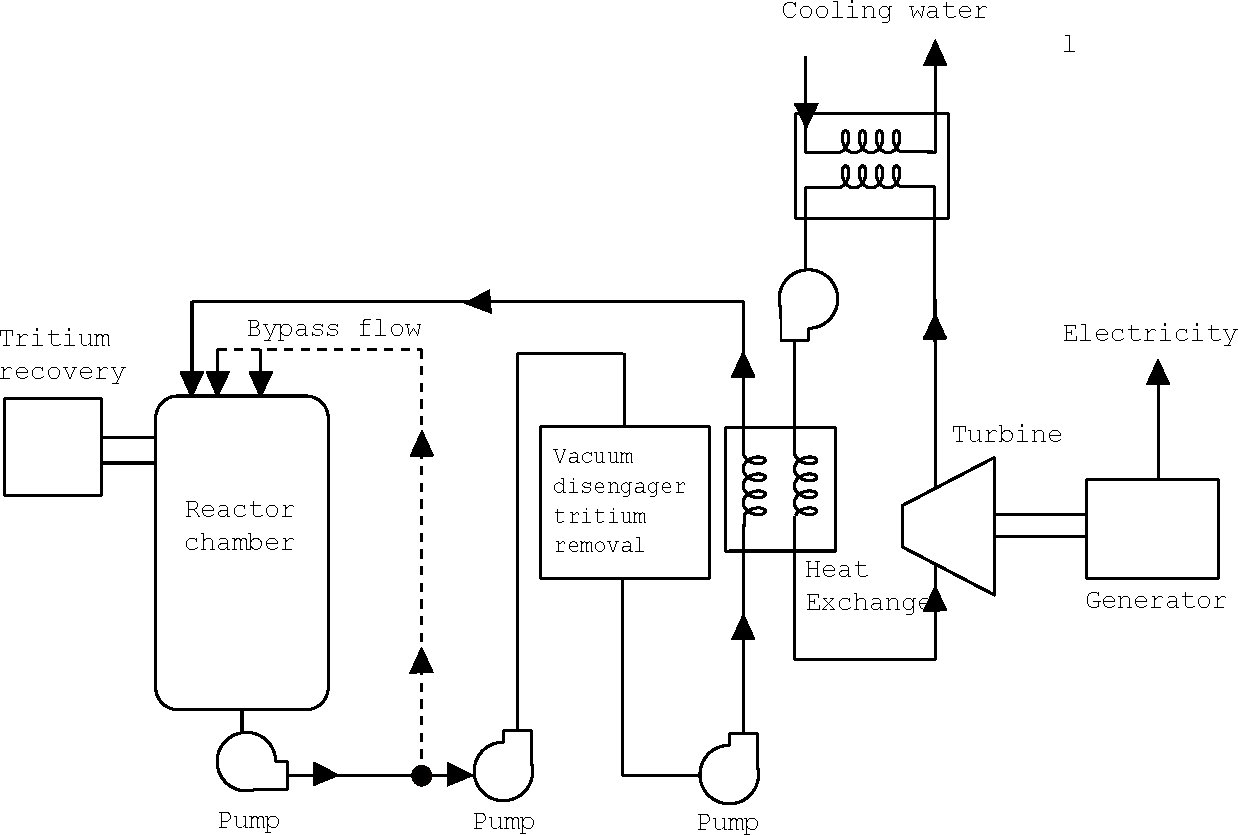
\includegraphics[width=0.8\linewidth]{StandardFigures/steamPbLi-eps-converted-to.pdf}
\caption{Main coolant system.}
\label{fig:coola}
\end{figure} 